%%%%%%%%%%%%%%%%%%%%%%%%%%EJERCICIO 10 %%%%%%%%%%%%%%%%%%%%%%%%%%%
 \textbf{Ejemplo 10}\\
	Resolver el problema anterior, suponiendo que el gradiente es escalonado con pagos semestrales.\\		
	
	\textbf{Solución 10}\\
	%La tabla ira centrada
	\begin{center}
		\renewcommand{\arraystretch}{1.5}% Margenes de las celdas
		%Creación de la cuadricula de 3 columnas
		\begin{longtable}[H]{|p{0.5\linewidth}|p{0.5\linewidth}|}
			%Creamos una linea horizontal
			\hline
			%Definimos el color de la primera fila
			\rowcolor[HTML]{FFB183}
			%%%%% INICIO ASIGNACIÓN período FOCAL %%%%%%%
			%%%%%%%%%% INICIO TITULO
			%Lo que se hace aquí es mezclar las 3 columnas en una sola
			\multicolumn{2}{|c|}{\cellcolor[HTML]{FFB183}\textbf{1. Asignación período focal}}   \\ \hline
			%%%%%%%%%% FIN TITULO
			%%%%% INICIO DECLARACIÓN DE VARIABLES %%%%%%%
			\multicolumn{2}{|c|}{$pf = 0 \textit{ psv}$}\\ \hline
			%%%%%%%%%% INICIO TITULO
			%Lo que se hace aquí es mezclar las 3 columnas en una sola
			\multicolumn{2}{|c|}{\cellcolor[HTML]{FFB183}\textbf{2. Declaración de variables}}   \\ \hline
			%%%%%%%%%% FIN TITULO
			%%%%%%%%%% INICIO DE MATEMÁTICAS
			%Cada & hace referencia al paso de la siguiente columna
			$VP = 500.000 \ COP $  				& $ n_{2}= 2 \hspace{1mm} psv $  \\
			$i \equiv  10\% \hspace{1mm} pav$      	& $ n_{3}= 3 \hspace{1mm} psv $ \\
			$ n = 2 \hspace{1mm} psv $          & $ n_{5}= 5 \hspace{1mm} psv $\\ 
			$ n_{1}= 1 \hspace{1mm} psv $       & $ n_{6}= 6 \hspace{1mm} psv $ \\ 
			$ $      						    & $ i \equiv  ? \% psv $ \\ \hline
			%%%%%%%%%% FIN DE MATEMÁTICAS
			%%%%% FIN DECLARACIÓN DE VARIABLES
			
			\rowcolor[HTML]{FFB183}
			\multicolumn{2}{|c|}{\cellcolor[HTML]{FFB183}\textbf{3. Diagrama de flujo de caja}} \\ \hline
			\multicolumn{2}{|c|}{ 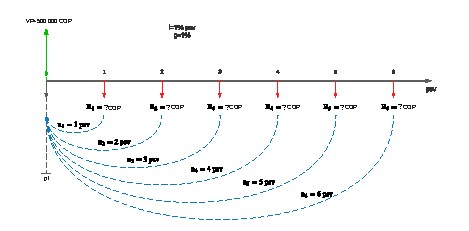
\includegraphics[trim=-78 -5 -78 -5]{7_Capitulo/img/ejemplos/10/10_1.pdf} }   \\ \hline
			%%%%% INICIO FLUJO DE CAJA
			\rowcolor[HTML]{FFB183}
			\multicolumn{2}{|c|}{\cellcolor[HTML]{FFB183}\textbf{4. Declaración de fórmulas}} \\ \hline
			%%%%%%%%%%%%% FIN INSERCIÓN DE IMAGEN
			%%%%%FIN FLUJO DE CAJA
			
			\multicolumn{2}{|c|}{ $(1+i_1)^{m_1} = (1+i_2)^{m_2} $ Equivalencia de tasas}   \\  
			\multicolumn{2}{|c|}{ $VF = R\frac{(1+i)^{n} -1 }{i} $ Valor presente serie uniforme}   \\  \hline
			
			%%%%%% INICIO DESARROLLO MATEMÁTICO
			\rowcolor[HTML]{FFB183}
			%%%%%%%%%%INICIO TITULO
			\multicolumn{2}{|c|}{\cellcolor[HTML]{FFB183}\textbf{5. Desarrollo matemático}}       \\ \hline
			%%%%%%%%%% FIN TITULO
			%%%%%%%%%% INICIO MATEMÁTICAS
			\multicolumn{2}{|c|}{  $(1+ 0,24)^{1} = (1+i)^{2} $}   \\ 
			\multicolumn{2}{|c|}{ $  i = 11,3552873\% \hspace{1mm} psv $}   \\  \hline
			
			%%%%%%%%%% FIN MATEMÁTICAS
			%%%%%% FIN DESARROLLO MATEMÁTICO
			%%%%%% INICIO RESPUESTA
			\rowcolor[HTML]{FFB183}
			%%%%%%%%%%INICIO TITULO
			\multicolumn{2}{|c|}{\cellcolor[HTML]{FFB183}\textbf{6. Respuesta}}   \\ \hline
			%%%%%%%%%% FIN TITULO
			%%%%%%%%%% INICIO RESPUESTA MATEMÁTICA
			\multicolumn{2}{|c|}{ 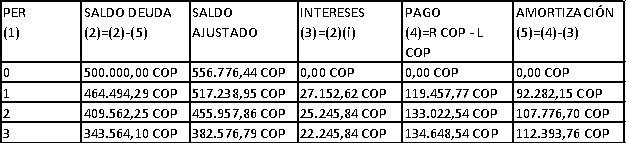
\includegraphics[trim=-78 -5 -78 -5]{7_Capitulo/img/ejemplos/10/10_2.pdf} }   \\ \hline
			%\multicolumn{2}{|C{\textwidth}|}{
			%	$R_{58} = 72.478,16 \ COP (1 + 0,02)^{57} = \ COP 224.087,15 $ 
			%}  \\ \hline
			
			
			%%%%%%%%%% FIN MATEMÁTICAS
			%%%%%% FIN RESPUESTA
		\end{longtable}
		%Se crean dos lineas en blanco para que no quede el siguiente texto tan pegado
		%\newline \newline %USARLO SI CREES QUE ES NECESARIO
	\end{center}
 %%%%%%%%%%%%%%%%%%%%%%%%%%FIN EJERCICIO 10 %%%%%%%%%%%%%%%%%%%%%%%%%%%